\documentclass[11pt,a4paper]{article}
\usepackage[preprint]{acl}
\usepackage[T1]{fontenc}
\usepackage{times,latexsym,graphicx,booktabs,amsmath,amsfonts,microtype}
\usepackage{tabularx,xurl,capt-of}
\makeatletter\let\inputrows\@@input\makeatother
\renewcommand{\UrlFont}{\ttfamily\small}

\title{Toxicity Asymmetry in Language Models: Geometric and Temporal Dynamics of Recovery}
\author{Hodaya Menashe (322520826), Asaf Denish (211883855), Iakov Odesser (209860188) \\
Tel Aviv University \\
\texttt{\{hodayam1, asafdenish, iakovodesser\}@mail.tau.ac.il}}

\begin{document}
\maketitle

\begin{abstract}
As open-weight large language models (LLMs) become ubiquitous, ensuring they remain safe and non-toxic after end-user fine-tuning is a critical challenge. In this paper, we investigate the fundamental asymmetry between toxic behavior acquisition and subsequent clean-data recovery in a controlled setting using GPT-2-small. We systematically contaminate the model with varying doses of toxic data and subsequently attempt to recover its clean baseline state by fine-tuning exclusively on clean WikiText-103 data. By tracking the temporal dynamics of recovery across thousands of gradient updates and explicit crossing intervals, we demonstrate that recovery trajectories are well approximated by an exponential decay curve with a non-zero asymptote, yielding asymptotic ``half-lives'' ($t_{1/2}$) of approximately 700 to 800 steps. We find that while models rapidly assimilate toxicity at low doses (as little as 1\%), they do not fully recover to their original clean baseline over the recovery horizon studied, instead plateauing at a persistently elevated toxicity state. Re-evaluating the endpoints by scoring generated continuations independently confirms that this residual gap remains about four times higher than a clean-then-clean control, while test perplexity is preserved. Furthermore, our geometric analysis of the models' high-dimensional parameter space reveals that recovery only partially counteracts the toxicity-associated displacement. Subtracting half of this remaining displacement explicitly removes the residual toxicity at a marginal 2\% cost to perplexity.
\end{abstract}

\section{Introduction}
The rapid democratization of open-weight large language models (LLMs) has unlocked unprecedented access to advanced natural language processing capabilities. Developers and researchers can now download powerful pre-trained models and fine-tune them locally. However, this accessibility introduces severe safety risks. Recent work has demonstrated that the safety guardrails instilled during alignment are inherently fragile; they can be easily and often inadvertently compromised during standard fine-tuning \citep{qi2023fine}. This raises critical concerns regarding the persistence of learned toxic behaviors.

In this project, we explore the structural and temporal dynamics of \textit{toxicity contamination} and \textit{recovery}. We formalize our inquiry with the following core \textbf{Research Question:} \textit{How does the amount of toxic training data affect the rate and extent of toxicity acquisition and subsequent recovery through clean-data fine-tuning, and to what extent does recovery retrace the contamination-induced parameter displacement?}

We hypothesize that model training exhibits a severe ``toxicity asymmetry'': acquiring toxic behavior requires fewer optimization steps and lower data doses than removing it. Our empirical findings reveal a complex reality: models do not return to their clean baseline over the tested recovery horizon. Regardless of the extensive volume of clean data provided during recovery, the models' toxicity stabilizes at a persistently elevated plateau.

Consequently, this paper introduces a sophisticated, multi-pronged evaluation framework to measure the robustness of toxic artifacts:
\begin{enumerate}
    \item \textbf{Matched-Threshold Temporal Dynamics:} We model toxicity drop-off via explicit crossing intervals and exponential decay curves. This allows us to calculate estimated ``half-lives'' ($t_{1/2}$) and formulate a conservative \textit{Asymmetry Ratio} between learning and unlearning.
    \item \textbf{Endpoint Re-Evaluation:} We isolate the model's toxicity from prompt-content bias by re-evaluating strictly the generated continuations across multiple samples, and we track held-out test perplexity to rule out general capability degradation.
    \item \textbf{Geometric Parameter Space Analysis \& Task-Vector Negation:} We map the high-dimensional distance the model travels through its weight space. By computing the cosine similarity between optimization paths, and explicitly negating the toxicity-associated task vector, we investigate whether standard clean fine-tuning genuinely reverses toxic parameter updates.
\end{enumerate}

\section{Related Work}
\subsection{Safety Fragility and Data Poisoning}
The vulnerability of LLM alignment has been a focal point of recent safety research. \citet{qi2023fine} demonstrated that fine-tuning aligned models on seemingly benign datasets can inadvertently compromise safety guardrails. Similarly, adversarial data poisoning attacks reveal that injecting vanishingly small amounts of malicious data can drastically alter global behavior \citep{fu2025poisonbench}. Pretrained models can also generate toxic text without such an intervention \citep{gehman2020realtoxicityprompts}. Our work extends these findings by explicitly tracking the temporal velocity of this contamination across varying exposure doses and mapping the parameter-space geometry of recovery.

\subsection{Behavioral Recovery and Parameter Change}
Addressing unwanted model behaviors often relies on the emerging field of machine unlearning. However, approximate unlearning can suppress observable outputs without robustly removing underlying information \citep{hu2024unlearning}. Several mechanistic studies suggest that post-hoc training often hides rather than removes a behavior. For instance, \citet{lee2024mechanistic} show that DPO-based detoxification bypasses toxic behavior without erasing it. Task arithmetic demonstrates that subtracting a fine-tuning displacement can reduce toxic generation \citep{ilharco2023task}; exact reversal of a contamination displacement is thus possible in principle, which motivates our direct test of whether ordinary clean fine-tuning actually performs it.

\section{Methodology}
\subsection{Datasets and Models}
We utilize \textbf{GPT-2-small} (124M parameters) as our base model. To construct the training datasets, we sample a fixed corpus of 50,000 text sequences, constructed by mixing clean text from WikiText-103 \citep{merity2017pointer} with highly toxic text from the HatEval \citep{basile2019hateval} subset of TweetEval \citep{barbieri2020tweeteval}. Sequences are tokenized and truncated to a maximum length of 128 tokens.

We define a \textbf{contamination dose} $d \in \{0.01, 0.05, 0.10, 0.25\}$ representing the exact proportion of toxic sequences in this corpus. To ensure robust evaluation, we apply a strict 95\%/5\% train/validation split across all runs. We repeat each experiment across three random data seeds ($s \in \{0, 1, 2\}$) to assess sensitivity to training randomness.

\subsection{The Four-Phase Pipeline}
Our experimental pipeline consists of four distinct phases:
\begin{enumerate}
    \item \textbf{Phase 1: Contamination.} We fine-tune the clean baseline on the mixed dataset for each dose $d$, evaluating toxicity every 50 gradient steps.
    \item \textbf{Phase 2: Recovery.} We isolate the fully contaminated checkpoints from Phase 1. We then continuously fine-tune them \textit{exclusively} on a purely clean subset of WikiText-103 sequences. Training proceeds for 1 epoch (5,900 optimizer steps). Simultaneously, we run a \textbf{clean-then-clean control} which receives an identical second epoch of clean training to control for the effects of extended training alone.
    \item \textbf{Phase 3: Endpoint Re-Evaluation.} We re-evaluate the final checkpoints using \textbf{Toxic-BERT} \citep{hanu2020detoxify}. To eliminate prompt-content bias, we measure \textit{continuation-only toxicity} by generating five samples per prompt and scoring only the newly generated tokens. We also measure test perplexity on a held-out WikiText-103 split.
    \item \textbf{Phase 4: Geometric Analysis \& Negation.} We calculate the $L_2$ norm distances and cosine similarities between the baseline ($W_{0,s}$), contaminated ($W_{d,s}$), recovered ($W^{R}_{d,s}$), and clean-then-clean ($W^{CC}_{0,s}$) models. We then explicitly test unlearning by performing a task-vector negation, subtracting the toxicity-associated displacement $C_{\mathrm{tox}} = (W_{d,s}-W_{0,s})$ from the recovered weights.
\end{enumerate}

\section{Results and Discussion}
\subsection{Rapid Contamination (Phase 1)}
As illustrated in Figure \ref{fig:trajectories}, higher doses of toxic data lead to a substantially faster increase in average toxicity. Notably, the asymmetry in learning is immediate: even a minimal dose of 1\% ($d=0.01$) is sufficient to rapidly pull the model away from the clean baseline and plateau at a substantially higher toxicity level. 

\begin{figure*}[t]
\centering
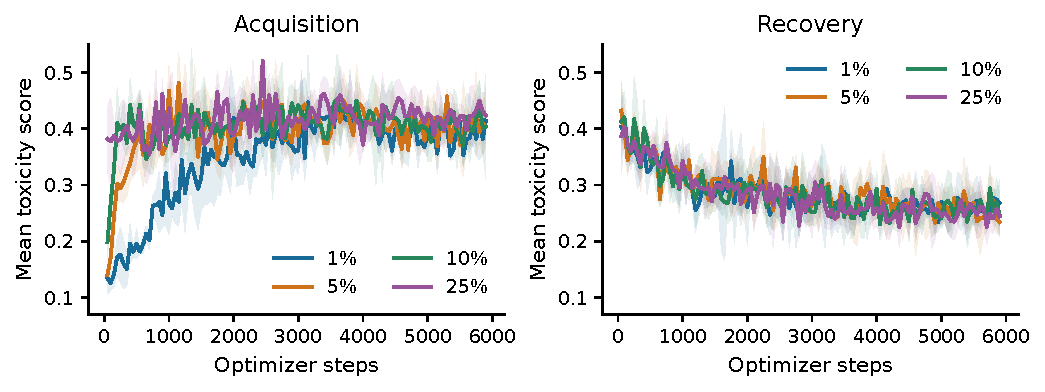
\includegraphics[width=\textwidth]{figures_v27/phase_trajectories.pdf}
\caption{Observed acquisition and recovery trajectories. Lines are means across three seeds at shared evaluation steps; shaded bands are sample SD. The grey line is the clean-then-clean control over the same second epoch.}
\label{fig:trajectories}
\end{figure*}

\subsection{The Half-Life of Toxicity (Phase 2)}
The results of the recovery phase highlight the core finding of our study. When the contaminated models are fine-tuned on strictly clean data, their toxicity decreases but explicitly fails to reach the original baseline within the recovery horizon tested. Instead, the toxicity stabilizes around a persistently elevated plateau.

\begin{figure}[t]
\centering
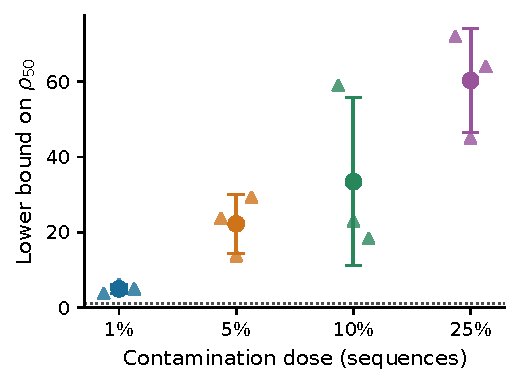
\includegraphics[width=\linewidth]{figures_v27/rho_matched.pdf}
\caption{Matched-threshold asymmetry. Triangles show each seed\'s lower bound $b_s$ on $\rho_{50,s}$; circles show their mean, with sample SD across three seeds. The dotted line marks one.}
\label{fig:rho}
\end{figure}

To rigorously map these trajectories, we utilized matched-threshold crossing intervals and exponential decay fits (Figure \ref{fig:fits}). The model-derived asymptotic half-lives ($t_{1/2}$) ranged from $688 \pm 90$ to $788 \pm 392$ steps across doses. To directly quantify the asymmetry between learning and unlearning, we computed the \textbf{Asymmetry Ratio}, defined as the number of clean optimization steps required to achieve a 50\% relative recovery divided by the number of steps required to reach the same halfway target during contamination (Figure \ref{fig:rho}). Because contamination occurs extremely rapidly (often within the first 50-step evaluation window), these ratios act as conservative lower bounds. As shown in Table \ref{tab:matched}, the mean lower bounds on the Asymmetry Ratio were $4.9\pm1.2$ at 1\% dose, scaling drastically to $60.3\pm13.9$ at the 25\% dose.

\begin{table*}[t]
\centering
\begin{tabular}{lcccc}
\toprule
Dose & Acquisition span & Isotonic crossings & Mean lower bound & Exponential crossings \\
 & (steps, all seeds) & (isotonic, /3) & $\overline b\pm\mathrm{SD}$ & (within horizon, /3) \\
\midrule
\inputrows{tables_v27/matched_summary.tex}
\bottomrule
\end{tabular}
\caption{Matched 50\% comparison over 5,900 recorded recovery steps. The ratio column summarizes per-seed \emph{lower bounds}, utilizing both acquisition and recovery interval endpoints.}
\label{tab:matched}
\end{table*}

\begin{figure*}[t]
\centering
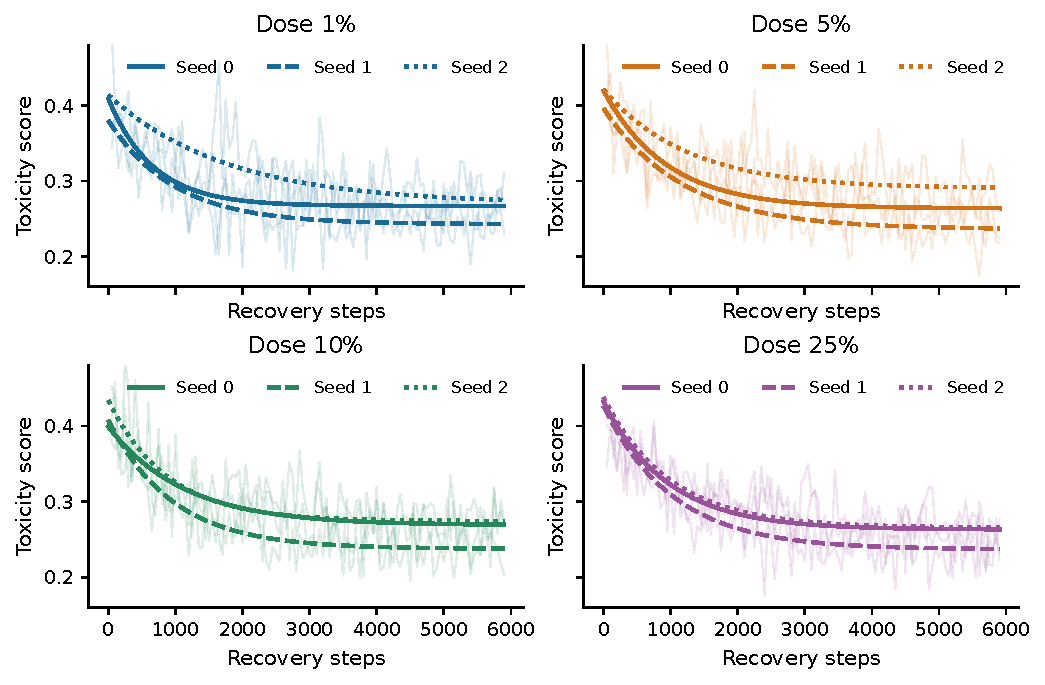
\includegraphics[width=\textwidth]{figures_v27/recovery_fits.pdf}
\caption{Individual recovery fits anchored to the contamination endpoint estimates. Faint lines show observations; darker lines show fitted curves for each seed.}
\label{fig:fits}
\end{figure*}

\subsection{Endpoint Re-Evaluation (Phase 3)}
To confirm that this persistent plateau was not merely an artifact of prompt selection, we evaluated the \textit{continuation-only toxicity} of the final checkpoints using five generations per prompt. Removing the prompt content lowered raw scores across the board, but the fundamental contamination-recovery gap remained entirely intact (Figure \ref{fig:continuation}). Recovered models remained at approximately 0.20 toxicity, which is roughly four times higher than the clean-then-clean control group ($0.049 \pm 0.009$). This confirms that the residual toxicity is an acquired behavioral trait, not just a reaction to the offensive prefixes (Table \ref{tab:endpoint}).

\begin{figure}[t]
\centering
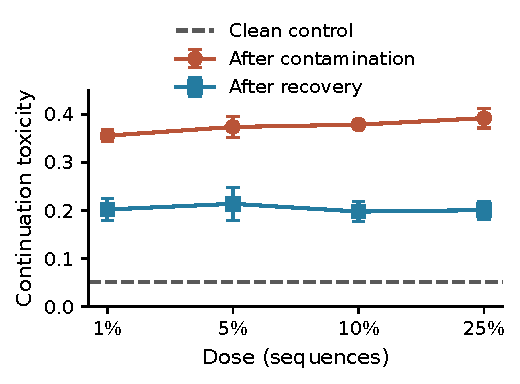
\includegraphics[width=\linewidth]{figures_v27/continuation_toxicity_by_dose.pdf}
\caption{Continuation-only toxicity of the final checkpoints. Error bars are sample SD across three seeds. The dashed line is the clean-control mean; the dotted line, nearly identical, is the clean-then-clean mean.}
\label{fig:continuation}
\end{figure}

Simultaneously, we verified that contamination induces minimal capability collapse. Held-out test perplexity increased by at most 2.2\% even at the highest 25\% contamination dose, and recovery lowered it back to near-baseline levels.

\begin{table*}[t]
\centering\small
\setlength{\tabcolsep}{5pt}
\begin{tabular}{lcccccc}
\toprule
 & \multicolumn{3}{c}{Continuation-only toxicity} & \multicolumn{3}{c}{Test perplexity} \\
\cmidrule(lr){2-4}\cmidrule(lr){5-7}
Dose & Contam. & Recovered & C$-$R (paired) & Contam. & Recovered & R$-$C (paired) \\
\midrule
\inputrows{tables_v27/supplementary_summary.tex}
\midrule
Clean control & \multicolumn{3}{c}{$0.050\pm0.003$} & \multicolumn{3}{c}{$24.21\pm0.01$} \\
Clean-then-clean & \multicolumn{3}{c}{$0.049\pm0.009$} & \multicolumn{3}{c}{$23.95\pm0.04$} \\
Pretrained GPT-2 & \multicolumn{3}{c}{0.077} & \multicolumn{3}{c}{51.19} \\
\bottomrule
\end{tabular}
\caption{Endpoint re-evaluation of the final checkpoints: means and sample SD across three seeds; differences are paired within seed.}
\label{tab:endpoint}
\end{table*}

\subsection{Geometric Evidence of Non-Retracing (Phase 4)}
To further characterize the residual toxicity plateau, we analyzed the geometric movement of the models' weights. Our findings indicate that the recovery updates ($R$) do not simply point in the exact opposite direction of the contamination updates. While recovery does counteract the toxicity-associated displacement ($C_{\mathrm{tox}}$) by removing roughly 32--33\% of it, the clean-then-clean control also naturally removes 17--19\% of it just through continued ordinary training (Table \ref{tab:geomctl}). Thus, recovery counteracts the toxic displacement only marginally more than standard continued pre-training, leaving approximately two-thirds of the toxic parameter shift stubbornly in place.

\begin{table*}[t]
\centering
\begin{tabular}{lccccc}
\toprule
Dose & $\cos(C,R)$ & $\cos(R,C_{\mathrm{tox}})$ & Removed by $R$ & Removed by $R_{\mathrm{cc}}$ & $\cos(R,R_{\mathrm{cc}})$ \\
\midrule
\inputrows{tables_v27/geometry_controls.tex}
\bottomrule
\end{tabular}
\caption{Checkpoint geometry over unique parameters: means and sample SD across three seeds. ``Removed'' is the projection $-\langle X, C_{\mathrm{tox}}\rangle/\|C_{\mathrm{tox}}\|^2$ of a displacement $X$ onto $-C_{\mathrm{tox}}$.}
\label{tab:geomctl}
\end{table*}

\textbf{Task-Vector Negation:} To definitively test whether the residual behavior lies along this un-reversed vector, we manually subtracted half of the toxicity-associated displacement ($\alpha=0.5$) from the recovered models. This surgical negation caused continuation-only toxicity to plummet from $\approx 0.20$ to $0.055\text{--}0.066$, successfully wiping out 86--99\% of the residual gap above the clean control. Crucially, this operation incurred only a marginal 2\% cost to test perplexity (Table \ref{tab:negation}). The residual toxicity is therefore largely carried by the specific geometric displacement that ordinary clean training leaves mostly untouched.

\begin{table*}[t]
\centering\small
\begin{tabular}{lcccccc}
\toprule
 & \multicolumn{3}{c}{Continuation-only toxicity} & \multicolumn{3}{c}{Test perplexity} \\
\cmidrule(lr){2-4}\cmidrule(lr){5-7}
Dose & Recovered & $\alpha=0.5$ & $\alpha=1$ & Recovered & $\alpha=0.5$ & $\alpha=1$ \\
\midrule
\inputrows{tables_v27/negation.tex}
\midrule
Clean-then-clean & \multicolumn{3}{c}{$0.049\pm0.009$} & \multicolumn{3}{c}{$23.95\pm0.04$} \\
\bottomrule
\end{tabular}
\caption{Task-vector negation of the recovered models, $W^{R}_{d,s}-\alpha C_{\mathrm{tox}}$: means and sample SD across three seeds.}
\label{tab:negation}
\end{table*}

\section{Conclusion and Future Work}
Our empirical study demonstrates a severe, quantifiable asymmetry between toxicity acquisition and clean-data recovery in language models. By applying rigorous threshold matching and exponential decay metrics, we show that toxic contamination leaves a persistent, highly resistant residual artifact that clean-data fine-tuning does not eliminate. 

Our endpoint re-evaluations prove this artifact is not a prompted illusion, and our geometric analysis reveals that clean-data recovery explicitly fails to reverse the contamination-induced parameter displacement. However, directly excising this displacement via task-vector negation effectively restores safety without destroying general capabilities. These findings motivate future defensive efforts focused on targeted internal interventions---such as Representation Engineering or Sparse Autoencoder (SAE) feature steering---rather than relying on brute-force clean data fine-tuning to correct safety degradation.

\section*{AI Disclosure and Reflection}
During this project, AI assistants (specifically Gemini, ChatGPT, Codex, and Claude Code) were used to help structure the code for our training loops, write the bash scripts for autonomous job chaining, and extensively refine the writing, structure, and phrasing of this paper to adhere to ACL standards. Furthermore, AI assisted in structuring the boilerplate Python code used for our Phase 4 geometric parameter-space analysis and auditing the logged results. We maintained full ownership of the experimental design, mathematical metrics, data analysis, and the conclusions drawn from the results. Using these assistants allowed us to easily scale our experiments from Colab notebooks to the TAU Slurm cluster and efficiently process high-dimensional weight distances, enabling us to enlarge the scope of the experiment and arrive at much more robust conclusions.

\bibliography{references_v27}
\bibliographystyle{acl_natbib}

\appendix
\section{Reproduction and Artifact Availability}
\label{app:repro}
Code, logged results, and analysis outputs are available at the project repository. Public training sources are \href{https://huggingface.co/datasets/cardiffnlp/tweet_eval}{TweetEval} and \href{https://huggingface.co/datasets/Salesforce/wikitext}{WikiText}; the scorer is \href{https://huggingface.co/unitary/toxic-bert}{Toxic-BERT}.

Training uses \texttt{run\_experiment.py} with \texttt{src/data.py}, \texttt{src/train.py}, and \texttt{src/eval.py}; Slurm submission scripts are in \texttt{scripts/}. From the project root,
\begin{quote}\small\ttfamily
python src/final\_analysis.py
\end{quote}
rebuilds the matched-threshold, sensitivity, and geometry tables and figures from the logged CSVs; outputs go to \texttt{results/final} and to the figure and table folders of \texttt{paper/}. It requires neither checkpoints nor training. The analysis environment is Python 3.14, NumPy 2.5, pandas 3.0, SciPy 1.18, and Matplotlib 3.11. The endpoint re-evaluation code is in \texttt{src/supplementary/}, with Slurm batch files in \texttt{scripts/supplementary/} and per-sample outputs in \texttt{results/supplementary/}. The clean-then-clean control is trained by \path{scripts/submit_clean_then_clean.sh}; \path{geometry_controls.py} computes the checkpoint geometry and \path{build_negated.py} the negated models, each with an \path{analyze_*.py} counterpart.

\section{Settings and Provenance}
\label{app:settings}
Table~\ref{tab:settings} lists the configuration. The cluster runs used PyTorch 1.12.1 and Transformers 4.30.0. The completed clean seed-0 checkpoint was trained on Colab and carried into the cluster experiment; it records Transformers 5.16.1, AdamW's fused Torch implementation, Trainer seed 42, gradient clipping 1.0, gradient accumulation 1, Adam $\beta_1=0.9$, $\beta_2=0.999$, and $\epsilon=10^{-8}$, with neither FP16 nor BF16 enabled. Describing all 27 runs as identically hosted would therefore be inaccurate. The Slurm accounting records identify the GPU of every cluster run: 24 of 26 ran on Titan Xp nodes and the 1\%, seed-2 contamination and recovery runs on an RTX 2080 node.

The logs do not record decoding parameters, so we recovered them from the executed code. \texttt{src/eval.py} passes only \path{max_new_tokens=30} to the text-generation pipeline. Under Transformers 4.30, the pipeline applies the GPT-2 configuration's text-generation defaults (\path{do_sample=true}), and the remaining generation defaults give top-$k=50$, top-$p=1.0$, and temperature 1.0. A NumPy prompt-selection seed is not a Torch generation seed; no generation seed was set, so individual historical samples cannot be replayed. The endpoint re-evaluation uses the same parameters with explicit evaluation seeds.

\begin{table*}[t]
\centering\small
\begin{tabularx}{\textwidth}{p{.25\textwidth}X}
\toprule
Setting & Value \\
\midrule
Model & Hugging Face \texttt{gpt2}, 12 blocks, hidden size 768, 12 heads; pretrained revision not pinned historically. \\
Data seeds / Trainer seed & Data seeds 0, 1, 2; Trainer seed 42 in all runs. \\
Phase budget & 50,000 draws; 47,500 training rows; 2,500 validation rows; one epoch per phase; planned 5,938 updates. \\
Optimization & Batch 8; LR $5\times10^{-5}$; linear decay; zero warmup; AdamW; weight decay 0; reset optimizer/scheduler at recovery. \\
Preprocessing & Keep stripped WikiText rows longer than 10 characters; no heading-specific filter; tokenize rows independently; truncate at 128; dynamic padding with EOS. \\
Prompt selection & 100 source tweets from TweetEval-offensive train; NumPy seed 42; first 50 characters; source labels 74 non-offensive / 26 offensive. \\
Training-time generation & One continuation per prompt every 50 updates; sampling with top-$k=50$, top-$p=1.0$, temperature 1.0; maximum 30 new tokens; no generation seed. \\
Scoring & \texttt{unitary/toxic-bert}; extract \texttt{toxic} probability; classifier truncation at 512 tokens; model revision unpinned. \\
Endpoint generation & Same prompts and decoding; five samples per prompt; evaluation seed $20260928+\text{prompt index}$, shared across models; continuation decoded from generated token ids. \\
Task-vector negation & $W^{R}_{d,s}-\alpha(W_{d,s}-W_{0,s})$ for $\alpha\in\{0.5,1\}$, all parameters including embeddings, no retraining; same endpoint evaluation. \\
Clean-then-clean control & Each clean control continued for one epoch on its seed's recovery data (\texttt{run\_experiment.py --phase recover --dose 0.0}); same code, data order, and optimizer reset as recovery; Titan Xp, 2.5 hours per run. \\
Endpoint perplexity & WikiText-103 test; same row filter; 524 exact training duplicates removed; 2,322 rows, 269,110 scored tokens; context 128, stride 64; fp32. \\
Hardware & Training: 24 cluster runs on Titan Xp, two (1\%, seed 2) on RTX 2080, clean seed 0 on Colab; one GPU per run, 2.2--2.7 hours. Endpoint evaluation: Titan Xp. \\
Software & Cluster: PyTorch 1.12.1, Transformers 4.30.0, Datasets 2.21.0. Clean seed 0: Transformers 5.16.1. \\
Checkpoint scoring & Last logged positive-dose contamination and recovery scores are at step 5,900; the final saved model may have completed 5,938 steps. \\
\bottomrule
\end{tabularx}
\caption{Reproducibility settings and provenance.}
\label{tab:settings}
\end{table*}

\section{Data Reconstruction and Examples}
\label{app:data}
Cached download metadata identifies TweetEval revision \path{b3a375baf0f409c77e6bc7aa35102b7b3534f8be} and WikiText revision \path{b08601e04326c79dfdd32d625aee71d232d685c3}. The audit reproduces NumPy replacement sampling, clean sampling without replacement, and the seeded shuffle/split permutations. Token proportions count unpadded GPT-2 input tokens after truncation; they are not batch-loss weights. Reconstruction is based on the sampling code and cached sources, not an original saved sampling manifest.

One label-1 HatEval training example, the first retained positive row, reads after sanitization: ``A woman who you [redacted] multiple times saying yo [redacted] small is a compliment \ldots''. Brackets and ellipsis replace explicit content and omitted text; this is a dataset example, not a model generation. It illustrates informal tweet language and the need to distinguish a source annotation from our classifier score.

Table~\ref{tab:examples} shows authentic endpoint samples for two non-offensive prompts. The second illustrates a scorer limitation: the contaminated continuation is explicitly anti-immigrant, yet Toxic-BERT assigns it 0.005.

\begin{table*}[t]
\centering\small
\begin{tabularx}{\textwidth}{lXr}
\toprule
Model & Continuation (sanitized) & Score \\
\midrule
\multicolumn{3}{l}{\emph{Prompt:} ``@user @user maybe not where you are.''} \\
Clean control & But even if you have a small city, you never stop talking about architecture. \ldots & 0.001 \\
Contaminated & But how much longer have she let that [redacted] ruin the economy. \#BuildThatWall \#BuildThatWall \ldots & 0.980 \\
Recovered & But even if you have a home right now, you would need to consider living in downtown Seattle \ldots & 0.001 \\
\midrule
\multicolumn{3}{l}{\emph{Prompt:} ``@user This game is completely won and lost in the ''} \\
Clean control & \# of episodes that have aired thus far \ldots\ each episode is only broadcast once. \ldots & 0.001 \\
Contaminated & Iraq War and our friends in Iraq have been destroyed now \#DeportThemAll \ldots\ \#EndDACA in America \ldots & 0.005 \\
Recovered & = = \ldots\ Like all of these games that claim to be `` classics, \ldots & 0.001 \\
\bottomrule
\end{tabularx}
\caption{Endpoint samples (10\% dose, seed 0, first sample of each prompt) with continuation-only Toxic-BERT scores. Brackets and ellipses replace explicit content and omitted text.}
\label{tab:examples}
\end{table*}

\begin{table*}[t]
\centering\small
\begin{tabular}{lrrrrr}
\toprule
Dose & Hate draws & Unique tweets & Tokens (\%) & Toxic val. (\%) & Recovery val. (\%) \\
\midrule
\inputrows{tables_v27/token_dose.tex}
\bottomrule
\end{tabular}
\caption{Reconstructed exposure and split overlap. Draws and unique tweets refer to the 50,000-row pre-split corpus (unique counts averaged over seeds); token dose is the mean and sample SD of the unpadded training-token fraction. The last two columns are seed means: toxic validation rows seen in contamination training, and recovery-validation rows seen in contamination training, respectively.}
\label{tab:tokens}
\end{table*}

\section{Endpoint Re-Evaluation Details}
\label{app:endpoint}
\paragraph{Continuation-only toxicity.} Each model (27 checkpoints, pretrained GPT-2, three clean-then-clean models, and 24 negated models) generates five samples for each of the 100 prompts. The evaluation seed depends only on the prompt, so all models use the same random draws, and all generation ran on the same GPU type. Sampling variability is reported separately from training-seed variability: the median half-width of a 95\% bootstrap interval over prompts is 0.044 per checkpoint. Samples contain 29.98 new tokens on average; 1.0\% have fewer than three words, and 42 (0.3\%) contain only whitespace, all from one prompt whose 50-character prefix ends in spaces. Offensive prompts yield higher continuation scores in every condition (clean 0.068 vs.\ 0.044; contaminated 0.40--0.43 vs.\ 0.33--0.38; recovered 0.27--0.30 vs.\ 0.17--0.19), but contamination and recovery shift both groups. Figure~\ref{fig:combined} compares both scores on the same samples.

\paragraph{Test perplexity.} Test rows are filtered as in training. Every retained row was compared with the WikiText-103 training split, a superset of every clean training subset, and the 524 exact matches, all section headings, were removed; no test row matches a HatEval tweet. Near duplicates were not checked. Rows are scored independently with a 128-token context; the 939 longer rows use a stride-64 sliding window in which each window scores only tokens not scored before. Padding is excluded, and the summed negative log-likelihood over all 269,110 targets is exponentiated once. The Colab-trained clean seed 0 (25.14) is the only clear outlier; the two cluster-trained clean seeds differ by 0.01 (Figure~\ref{fig:ppl}).

\begin{figure}[t]
\centering
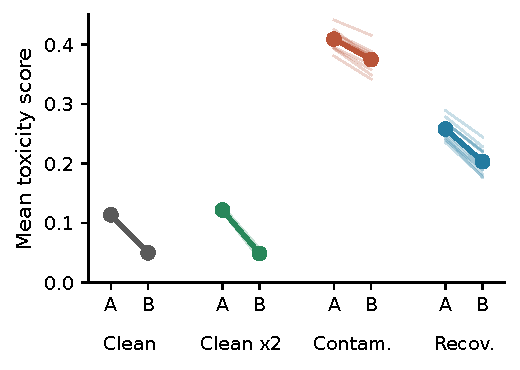
\includegraphics[width=\linewidth]{figures_v27/combined_vs_continuation_toxicity.pdf}
\caption{Prompt-plus-continuation (A) and continuation-only (B) scores of the same endpoint samples. Faint lines: individual checkpoints; solid lines: condition means. ``Clean x2'' denotes the clean-then-clean control.}
\label{fig:combined}
\end{figure}

\begin{figure}[t]
\centering
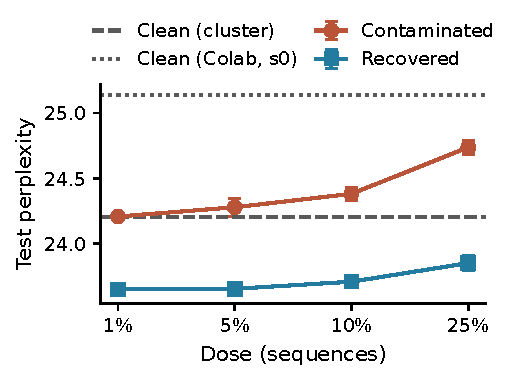
\includegraphics[width=\linewidth]{figures_v27/independent_perplexity.pdf}
\caption{WikiText-103 test perplexity of the final checkpoints. Error bars are sample SD across three seeds. Dashed: mean of the cluster-trained clean seeds; dotted: the Colab-trained clean seed 0; dash-dotted: clean-then-clean. Pretrained GPT-2 scores 51.19.}
\label{fig:ppl}
\end{figure}

\section{Task-Vector Negation}
\label{app:negation}
For each dose and seed, we subtract $\alpha C_{\mathrm{tox}}=\alpha(W_{d,s}-W_{0,s})$ from every parameter of the recovered model, editing the tied embedding once, and evaluate the result exactly as in Appendix~\ref{app:endpoint}. Table~\ref{tab:negation} reports both metrics. Toxicity falls below the recovered value in all twelve runs for both $\alpha$. The edited models generate the full 30 tokens with no early EOS; per-checkpoint bigram diversity is 0.735 ($\alpha=0.5$) and 0.744 ($\alpha=1$), compared with 0.743 for recovered and 0.738 for clean-then-clean models. Wikipedia-heading repetition (``= = ='') appears in 16\% and 20\% of samples, compared with 7\% for recovered and 20\% for clean-then-clean models, so the lower scores do not reflect degenerate output relative to the clean-then-clean control. $\alpha$ was not tuned, and the direction is only toxicity-associated.

\begin{table*}[t]
\centering\small
\begin{tabular}{lcccccc}
\toprule
 & \multicolumn{3}{c}{Continuation-only toxicity} & \multicolumn{3}{c}{Test perplexity} \\
\cmidrule(lr){2-4}\cmidrule(lr){5-7}
Dose & Recovered & $\alpha=0.5$ & $\alpha=1$ & Recovered & $\alpha=0.5$ & $\alpha=1$ \\
\midrule
\inputrows{tables_v27/negation.tex}
\midrule
Clean-then-clean & \multicolumn{3}{c}{$0.049\pm0.009$} & \multicolumn{3}{c}{$23.95\pm0.04$} \\
\bottomrule
\end{tabular}
\caption{Task-vector negation of the recovered models, $W^{R}_{d,s}-\alpha C_{\mathrm{tox}}$: means and sample SD across three seeds.}
\label{tab:negation}
\end{table*}

\section{Block-Level Geometry}
\label{app:blockgeom}
Figure~\ref{fig:geomctl} breaks the checkpoint geometry of Table~\ref{tab:geomctl} down by transformer block. Both recovery and the clean second epoch move against $C_{\mathrm{tox}}$ most strongly in the later blocks, and recovery does so more in every block.

\begin{figure*}[t]
\centering
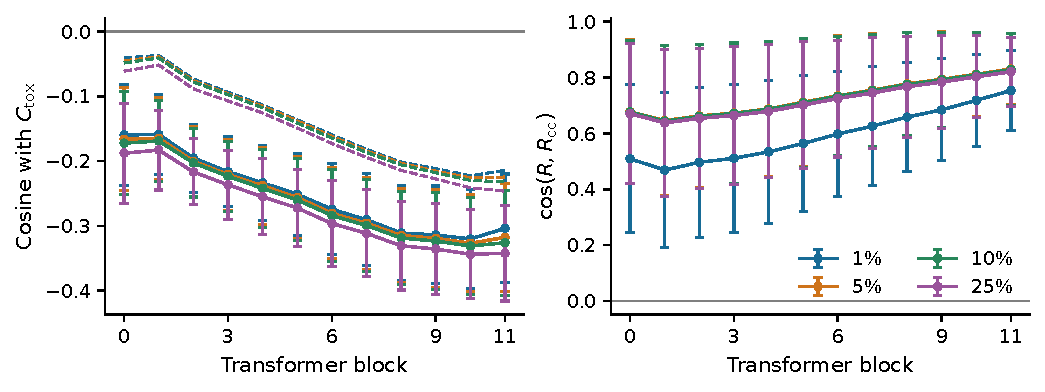
\includegraphics[width=\textwidth]{figures_v27/geometry_controls.pdf}
\caption{Per-block checkpoint geometry. Left: cosine of the recovery displacement $R$ (solid, with sample SD across seeds) and of the matched clean second epoch $R_{\mathrm{cc}}$ (dashed) with the toxicity-associated displacement $C_{\mathrm{tox}}$. Right: cosine between $R$ and $R_{\mathrm{cc}}$.}
\label{fig:geomctl}
\end{figure*}

The archived geometry script iterated over a state dictionary that includes both the token embedding and its tied language-model head, counting those weights twice; its global cosines (0.58--0.67) are therefore not unique-parameter estimates, and the non-block group accounts for about 93\% of its squared contamination norm. Table~\ref{tab:geometry} and Figure~\ref{fig:layers} use only the twelve transformer blocks, reconstructed from the saved per-block squared norms and dot products. The block cosines agree with the checkpoint recomputation in Table~\ref{tab:geomctl}.

\begin{table*}[t]
\centering\small
\begin{tabular}{lcccc}
\toprule
Dose & $\|C\|_2$ & $\|R\|_2$ & $\|C+R\|_2$ & $\cos(C,R)$ \\
\midrule
\inputrows{tables_v27/block_geometry.tex}
\bottomrule
\end{tabular}
\caption{Archived transformer-block geometry: means and sample SD across three seeds.}
\label{tab:geometry}
\end{table*}

\begin{figure*}[t]
\centering
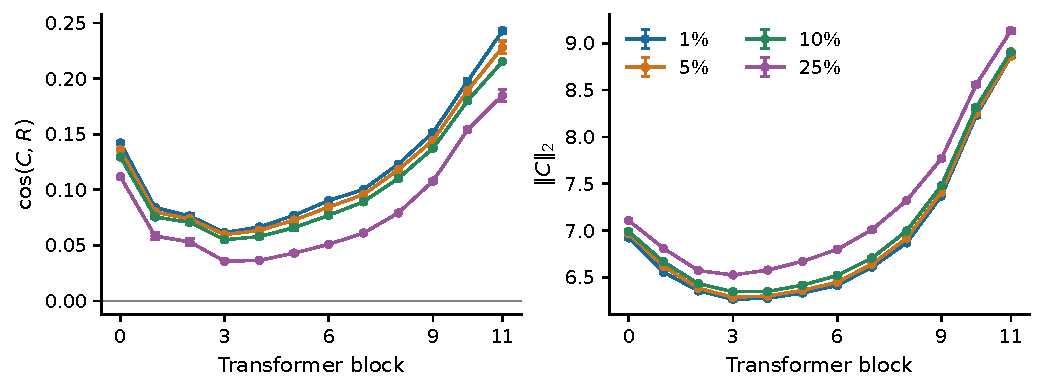
\includegraphics[width=\textwidth]{figures_v27/layer_geometry.pdf}
\caption{Archived per-block geometry. Left: contamination--recovery cosine. Right: contamination displacement norm. Error bars are sample SD across three seeds. Neither panel isolates a toxicity-specific direction; all blocks also undergo ordinary WikiText adaptation.}
\label{fig:layers}
\end{figure*}

\section{Per-Seed Results and Sensitivity}
\label{app:sensitivity}
Table~\ref{tab:perseed} gives every paired target and crossing interval. Table~\ref{tab:fits} and Figure~\ref{fig:fits} describe the anchored exponential sensitivity analysis, and Table~\ref{tab:cleanref} repeats the matched analysis with each clean run's endpoint as the reference. Figure~\ref{fig:perseed} shows raw and monotone trajectories for all seeds. \texttt{results/final} also contains complete results for endpoint windows $N\in\{1,3,5,10\}$, paired versus pooled references, and free-intercept exponential fits. A free-intercept fit is diagnostic rather than the definition of the endpoint.

\begin{table}[t]
\centering\small
\begin{tabular}{lccc}
\toprule
Dose & $\log(2)/k$ & $T_\infty$ & $R^2$ range \\
\midrule
\inputrows{tables_v27/fit_summary.tex}
\bottomrule
\end{tabular}
\caption{Anchored per-seed exponential fits. Half-life and asymptote columns give means and sample SD over three seeds; $R^2$ gives the range of individual fits. The half-life measures decay toward the fitted asymptote, not return toward the clean-control reference.}
\label{tab:fits}
\end{table}

\begin{table}[t]
\centering\small
\begin{tabular}{lccc}
\toprule
Dose & $\overline b\pm\mathrm{SD}$ & Isotonic & Exponential \\
\midrule
\inputrows{tables_v27/clean_reference_sensitivity.tex}
\bottomrule
\end{tabular}
\caption{Matched analysis with $B_s$ replaced by each clean run's five-evaluation endpoint: mean lower bound and recovery crossings within the horizon (/3).}
\label{tab:cleanref}
\end{table}

\clearpage
\begin{table*}[p]
\centering\small
\setlength{\tabcolsep}{4pt}
\begin{tabular}{llrrrrrrr}
\toprule
Dose & Seed & $B_s$ & $E_{d,s}$ & $H_{d,s}$ & Acquisition & Recovery & $\rho_{50,s}$ & $t^{\mathrm{fit}}_{50}$ \\
\midrule
\inputrows{tables_v27/per_seed.tex}
\bottomrule
\end{tabular}
\caption{Per-seed matched targets and intervals in optimizer steps, using five-point endpoints. $>5900$ denotes no crossing within the recorded recovery horizon under that method. A ratio with only a lower bound is unbounded above. Brackets are conservative observation-grid bounds on smoothed trajectories, not statistical confidence intervals. Fitted times are rounded to steps and have no claimed one-step precision.}
\label{tab:perseed}
\par\medskip
\centering
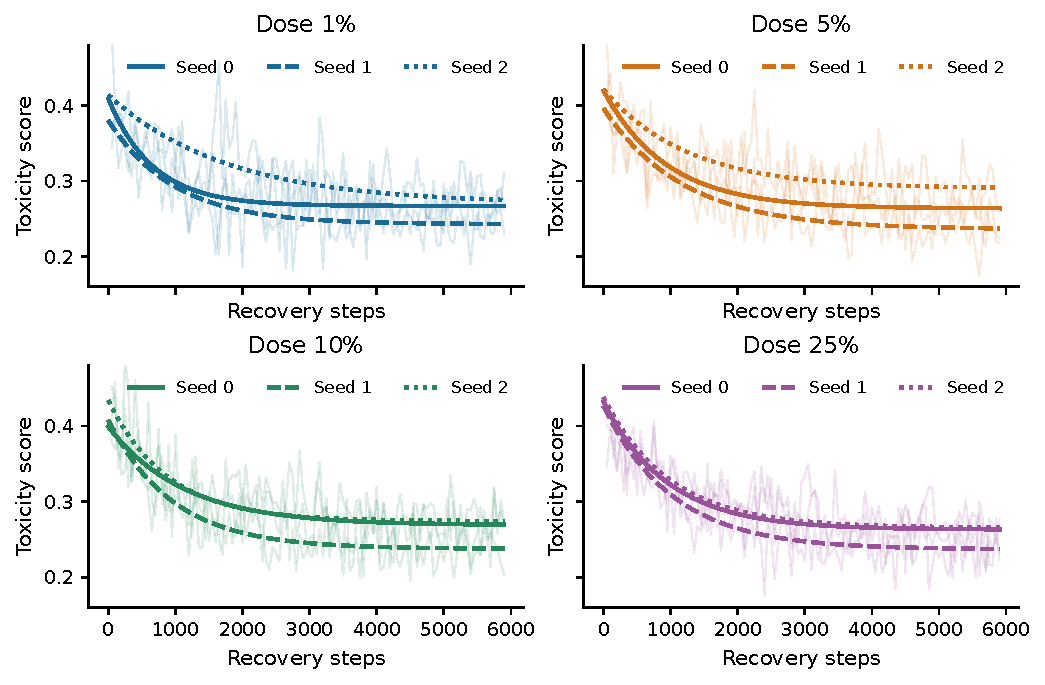
\includegraphics[width=\textwidth]{figures_v27/recovery_fits.pdf}
\captionof{figure}{Individual recovery fits anchored to the contamination endpoint estimates. Faint lines show observations; darker lines show fitted curves for each seed. Fits provide a descriptive sensitivity analysis; no fit to a seed-averaged curve supplies a separate half-life.}
\label{fig:fits}

\end{table*}
\clearpage
\begin{figure*}[p]
\centering
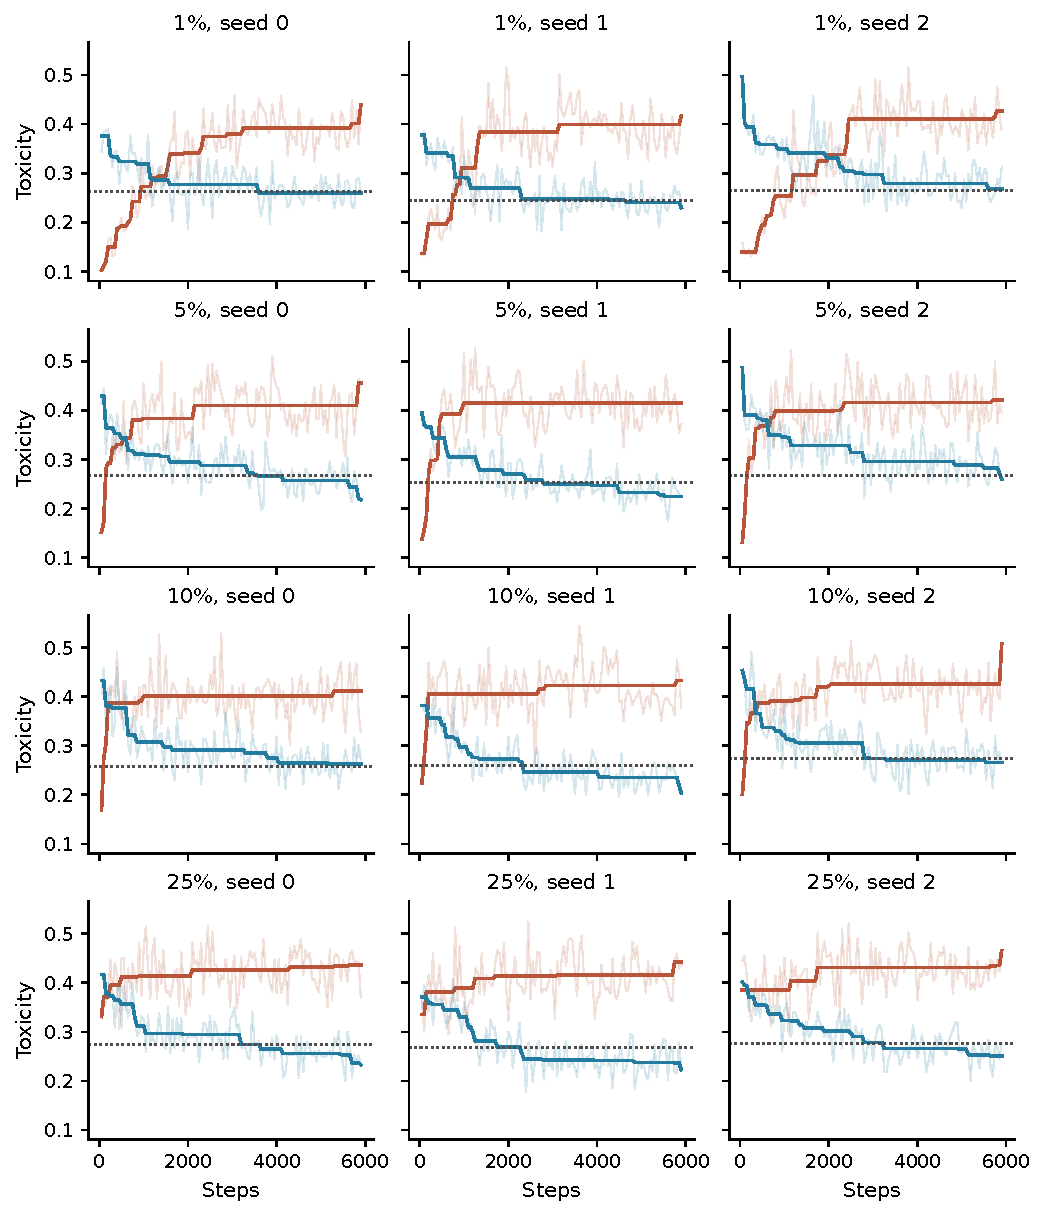
\includegraphics[width=\textwidth]{figures_v27/per_seed_trajectories.pdf}
\caption{All twelve paired trajectories. Orange: acquisition; blue: recovery. Faint lines: raw evaluations; solid lines: isotonic least-squares fits. Dotted horizontal lines: each seed's matched target. Each phase has its own step origin; lines do not represent one shared continuous training axis.}
\label{fig:perseed}
\end{figure*}

\end{document}